\documentclass{standalone}
\usepackage{tikz}
\usetikzlibrary{patterns, positioning}
\usepackage[sfdefault]{ClearSans} %% option 'sfdefault' activates Clear Sans as the default text font
\usepackage[T1]{fontenc}

\begin{document}
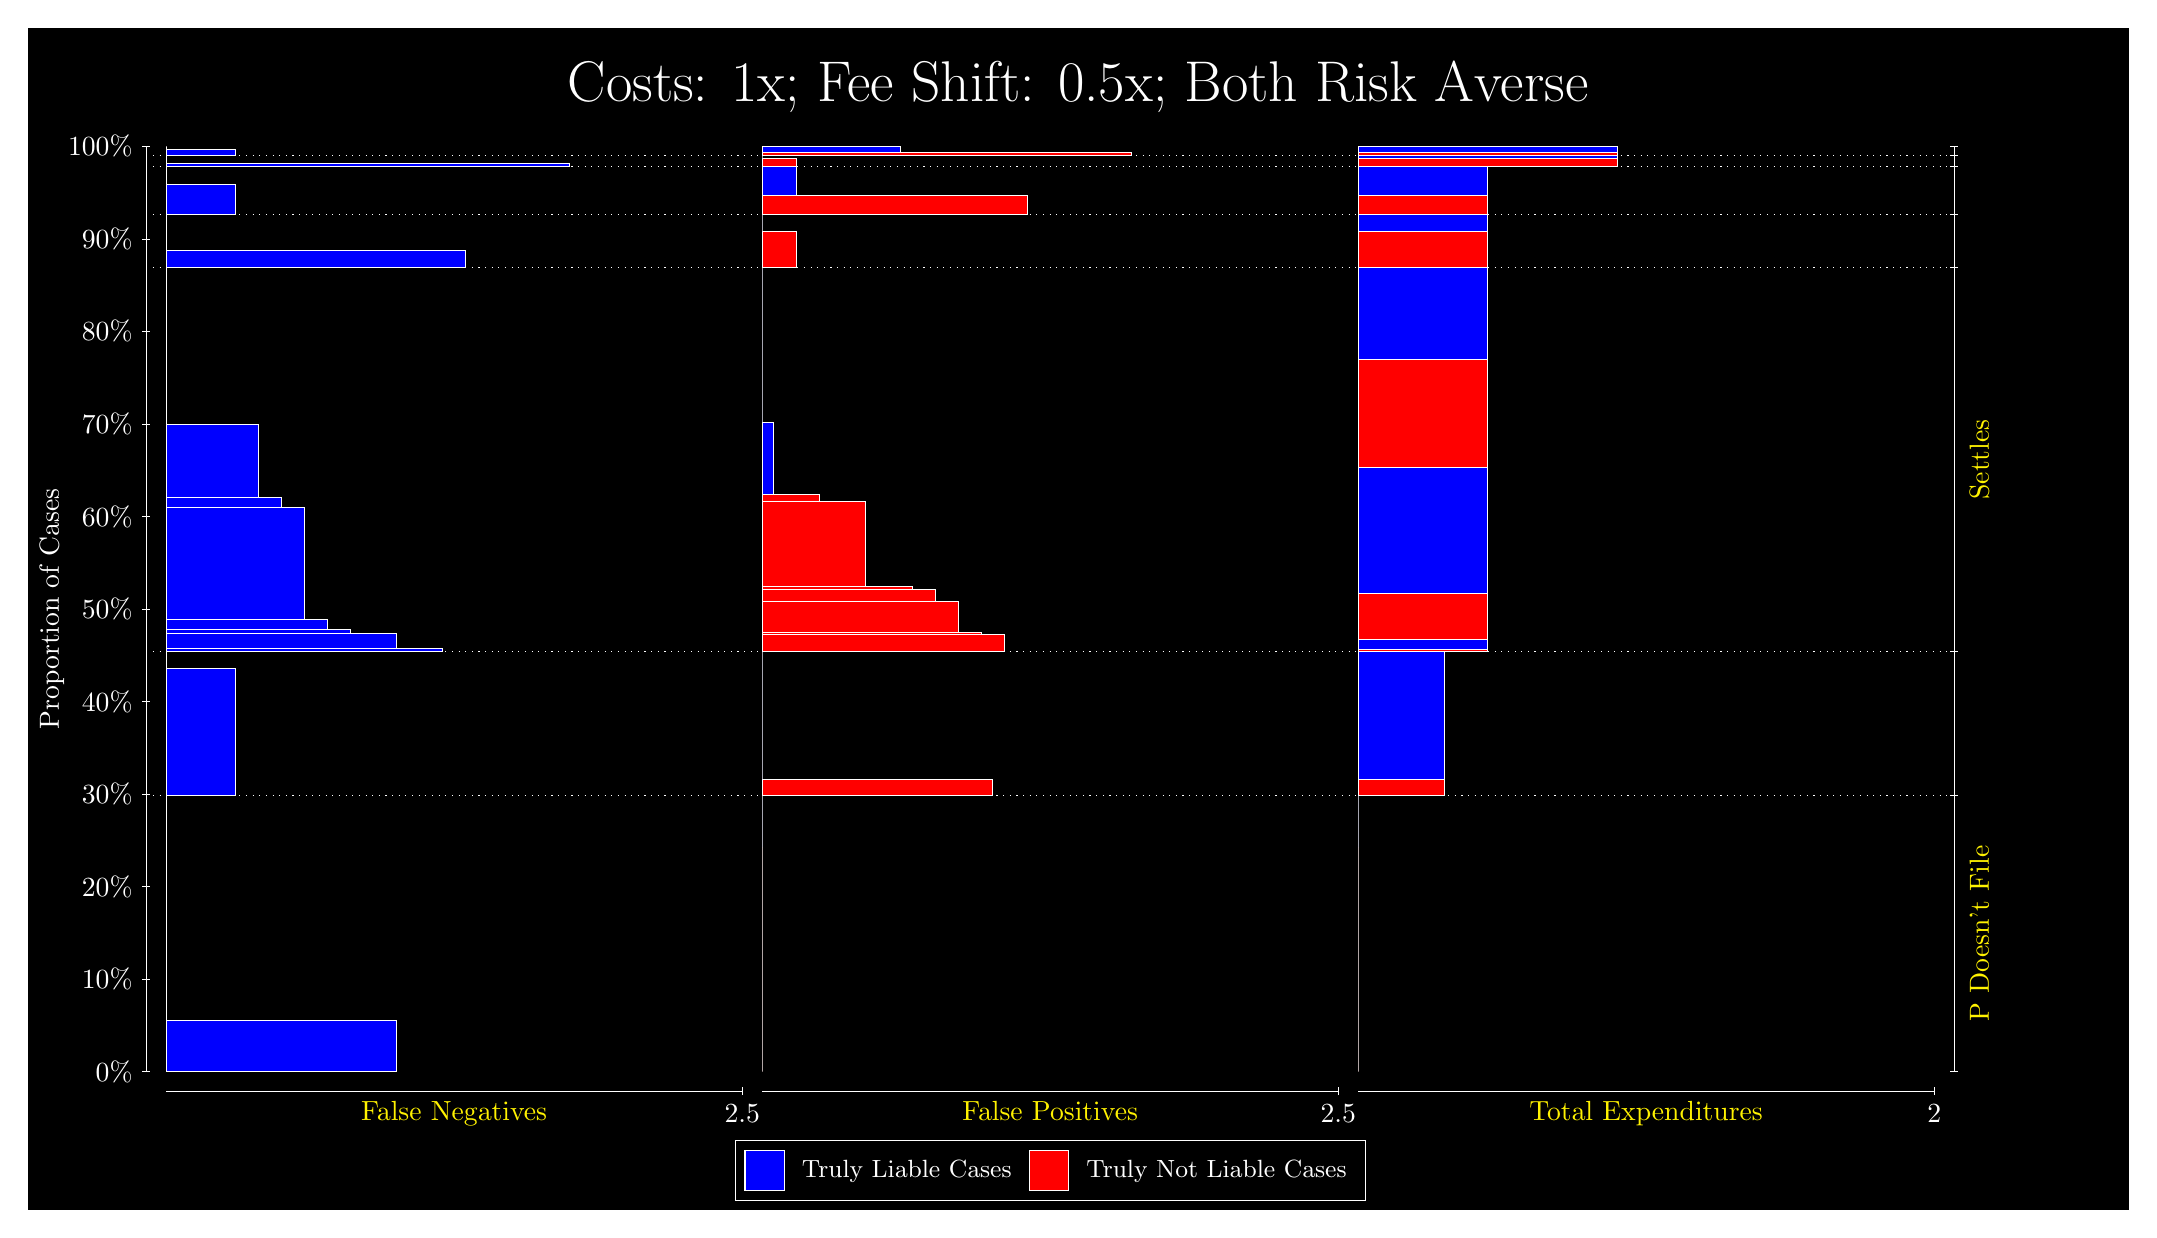
\begin{tikzpicture}
\draw[fill=black] (0,0) rectangle (26.667,15);
\draw[text=white] (0,13.5) rectangle (26.667,15) node[midway] {\huge Costs: 1x; Fee Shift: 0.5x; Both Risk Averse};
\draw[white, very thin] (1.5,1.75) -- (1.5,13.5);
\node[rotate=90, text=white, anchor=center] at (0.3, 7.625) {Proportion of Cases};
\draw[white, very thin] (1.45,1.75) -- (1.55,1.75);
\node[text=white, anchor=east] at (1.45, 1.75) {0\%};
\draw[white, very thin] (1.45,2.925) -- (1.55,2.925);
\node[text=white, anchor=east] at (1.45, 2.925) {10\%};
\draw[white, very thin] (1.45,4.1) -- (1.55,4.1);
\node[text=white, anchor=east] at (1.45, 4.1) {20\%};
\draw[white, very thin] (1.45,5.275) -- (1.55,5.275);
\node[text=white, anchor=east] at (1.45, 5.275) {30\%};
\draw[white, very thin] (1.45,6.45) -- (1.55,6.45);
\node[text=white, anchor=east] at (1.45, 6.45) {40\%};
\draw[white, very thin] (1.45,7.625) -- (1.55,7.625);
\node[text=white, anchor=east] at (1.45, 7.625) {50\%};
\draw[white, very thin] (1.45,8.8) -- (1.55,8.8);
\node[text=white, anchor=east] at (1.45, 8.8) {60\%};
\draw[white, very thin] (1.45,9.975) -- (1.55,9.975);
\node[text=white, anchor=east] at (1.45, 9.975) {70\%};
\draw[white, very thin] (1.45,11.15) -- (1.55,11.15);
\node[text=white, anchor=east] at (1.45, 11.15) {80\%};
\draw[white, very thin] (1.45,12.325) -- (1.55,12.325);
\node[text=white, anchor=east] at (1.45, 12.325) {90\%};
\draw[white, very thin] (1.45,13.5) -- (1.55,13.5);
\node[text=white, anchor=east] at (1.45, 13.5) {100\%};

\draw[white, very thin] (24.457,1.75) -- (24.457,13.5);
\draw[white, very thin] (24.407,1.75) -- (24.507,1.75);
\node[anchor=west] at (24.407, 1.75) {};
\draw[white, very thin] (24.407,5.2545) -- (24.507,5.2545);
\node[anchor=west] at (24.407, 5.2545) {};
\draw[white, very thin] (24.407,7.084) -- (24.507,7.084);
\node[anchor=west] at (24.407, 7.084) {};
\draw[white, very thin] (24.407,11.959) -- (24.507,11.959);
\node[anchor=west] at (24.407, 11.959) {};
\draw[white, very thin] (24.407,12.639) -- (24.507,12.639);
\node[anchor=west] at (24.407, 12.639) {};
\draw[white, very thin] (24.407,13.248) -- (24.507,13.248);
\node[anchor=west] at (24.407, 13.248) {};
\draw[white, very thin] (24.407,13.386) -- (24.507,13.386);
\node[anchor=west] at (24.407, 13.386) {};
\draw[white, very thin] (24.407,13.5) -- (24.507,13.5);
\node[anchor=west] at (24.407, 13.5) {};

\draw[white, very thin, fill=blue] (1.75,1.75) rectangle (4.6775,2.4058);
\draw[white, very thin, fill=red] (1.75,2.4058) rectangle (1.75,5.2545);
\draw[white, very thin, fill=blue] (1.75,5.2545) rectangle (2.6283,6.8774);
\draw[white, very thin, fill=red] (1.75,6.8774) rectangle (1.75,7.084);
\draw[white, very thin, fill=blue] (1.75,7.084) rectangle (5.2631,7.1205);
\draw[white, very thin, fill=blue] (1.75,7.1205) rectangle (4.6775,7.3186);
\draw[white, very thin, fill=blue] (1.75,7.3186) rectangle (4.3848,7.3214);
\draw[white, very thin, fill=blue] (1.75,7.3214) rectangle (4.092,7.3705);
\draw[white, very thin, fill=blue] (1.75,7.3705) rectangle (3.7993,7.4931);
\draw[white, very thin, fill=blue] (1.75,7.4931) rectangle (3.5065,8.9211);
\draw[white, very thin, fill=blue] (1.75,8.9211) rectangle (3.2138,9.0461);
\draw[white, very thin, fill=blue] (1.75,9.0461) rectangle (2.921,9.9683);
\draw[white, very thin, fill=red] (1.75,9.9683) rectangle (1.75,11.959);
\draw[white, very thin, fill=blue] (1.75,11.959) rectangle (5.5558,12.183);
\draw[white, very thin, fill=red] (1.75,12.183) rectangle (1.75,12.639);
\draw[white, very thin, fill=blue] (1.75,12.639) rectangle (2.6283,13.013);
\draw[white, very thin, fill=red] (1.75,13.013) rectangle (1.75,13.248);
\draw[white, very thin, fill=blue] (1.75,13.248) rectangle (6.8732,13.287);
\draw[white, very thin, fill=red] (1.75,13.287) rectangle (1.75,13.386);
\draw[white, very thin, fill=blue] (1.75,13.386) rectangle (2.6283,13.461);
\draw[white, very thin, fill=red] (1.75,13.461) rectangle (1.75,13.5);
\draw[white, very thin, fill=red] (9.3189,1.75) rectangle (9.3189,4.5988);
\draw[white, very thin, fill=blue] (9.3189,4.5988) rectangle (9.3189,5.2545);
\draw[white, very thin, fill=red] (9.3189,5.2545) rectangle (12.246,5.4612);
\draw[white, very thin, fill=blue] (9.3189,5.4612) rectangle (9.3189,7.084);
\draw[white, very thin, fill=red] (9.3189,7.084) rectangle (12.393,7.2982);
\draw[white, very thin, fill=red] (9.3189,7.2982) rectangle (12.1,7.33);
\draw[white, very thin, fill=red] (9.3189,7.33) rectangle (11.807,7.7181);
\draw[white, very thin, fill=red] (9.3189,7.7181) rectangle (11.515,7.8703);
\draw[white, very thin, fill=red] (9.3189,7.8703) rectangle (11.222,7.9113);
\draw[white, very thin, fill=red] (9.3189,7.9113) rectangle (10.929,7.9141);
\draw[white, very thin, fill=red] (9.3189,7.9141) rectangle (10.636,8.9935);
\draw[white, very thin, fill=red] (9.3189,8.9935) rectangle (10.051,9.0749);
\draw[white, very thin, fill=blue] (9.3189,9.0749) rectangle (9.4652,9.9971);
\draw[white, very thin, fill=blue] (9.3189,9.9971) rectangle (9.3189,11.959);
\draw[white, very thin, fill=red] (9.3189,11.959) rectangle (9.758,12.415);
\draw[white, very thin, fill=blue] (9.3189,12.415) rectangle (9.3189,12.639);
\draw[white, very thin, fill=red] (9.3189,12.639) rectangle (12.686,12.874);
\draw[white, very thin, fill=blue] (9.3189,12.874) rectangle (9.758,13.248);
\draw[white, very thin, fill=red] (9.3189,13.248) rectangle (9.758,13.347);
\draw[white, very thin, fill=blue] (9.3189,13.347) rectangle (9.3189,13.386);
\draw[white, very thin, fill=red] (9.3189,13.386) rectangle (14.003,13.425);
\draw[white, very thin, fill=blue] (9.3189,13.425) rectangle (11.075,13.5);
\draw[white, very thin, fill=red] (16.888,1.75) rectangle (16.888,4.5988);
\draw[white, very thin, fill=blue] (16.888,4.5988) rectangle (16.888,5.2545);
\draw[white, very thin, fill=red] (16.888,5.2545) rectangle (17.986,5.4612);
\draw[white, very thin, fill=blue] (16.888,5.4612) rectangle (17.986,7.084);
\draw[white, very thin, fill=red] (16.888,7.084) rectangle (18.534,7.1158);
\draw[white, very thin, fill=blue] (16.888,7.1158) rectangle (18.534,7.2407);
\draw[white, very thin, fill=red] (16.888,7.2407) rectangle (18.534,7.8221);
\draw[white, very thin, fill=blue] (16.888,7.8221) rectangle (18.534,9.4218);
\draw[white, very thin, fill=red] (16.888,9.4218) rectangle (18.534,10.8);
\draw[white, very thin, fill=blue] (16.888,10.8) rectangle (18.534,11.959);
\draw[white, very thin, fill=red] (16.888,11.959) rectangle (18.534,12.415);
\draw[white, very thin, fill=blue] (16.888,12.415) rectangle (18.534,12.639);
\draw[white, very thin, fill=red] (16.888,12.639) rectangle (18.534,12.874);
\draw[white, very thin, fill=blue] (16.888,12.874) rectangle (18.534,13.248);
\draw[white, very thin, fill=red] (16.888,13.248) rectangle (20.181,13.347);
\draw[white, very thin, fill=blue] (16.888,13.347) rectangle (20.181,13.386);
\draw[white, very thin, fill=red] (16.888,13.386) rectangle (20.181,13.425);
\draw[white, very thin, fill=blue] (16.888,13.425) rectangle (20.181,13.5);
\draw[white, dotted] (1.5,5.2545) -- (24.457,5.2545);
\draw[white, dotted] (1.5,7.084) -- (24.457,7.084);
\draw[white, dotted] (1.5,11.959) -- (24.457,11.959);
\draw[white, dotted] (1.5,12.639) -- (24.457,12.639);
\draw[white, dotted] (1.5,13.248) -- (24.457,13.248);
\draw[white, dotted] (1.5,13.386) -- (24.457,13.386);
\draw[white, very thin] (1.75,1.5) -- (9.0689,1.5);
\node[text=yellow, anchor=north] at (5.4094, 1.5) {False Negatives};
\draw[white, very thin] (9.0689,1.45) -- (9.0689,1.55);
\node[text=white, anchor=north] at (9.0689, 1.45) {2.5};

\draw[white, very thin] (9.3189,1.5) -- (16.638,1.5);
\node[text=yellow, anchor=north] at (12.978, 1.5) {False Positives};
\draw[white, very thin] (16.638,1.45) -- (16.638,1.55);
\node[text=white, anchor=north] at (16.638, 1.45) {2.5};

\draw[white, very thin] (16.888,1.5) -- (24.207,1.5);
\node[text=yellow, anchor=north] at (20.547, 1.5) {Total Expenditures};
\draw[white, very thin] (24.207,1.45) -- (24.207,1.55);
\node[text=white, anchor=north] at (24.207, 1.45) {2};

\node[text=yellow, centered, rotate=90] at (24.777, 3.5023) {P Doesn't File};

\node[text=yellow, centered, rotate=90] at (24.777, 9.5216) {Settles};





\draw (12.978300999999998,1.5) node[draw=none] (baseCoordinate) {};
\begin{scope}[align=center]
        \matrix[scale=0.5, draw=white, below=0.5cm of baseCoordinate, nodes={draw}, column sep=0.1cm]{
            \node[rectangle, draw, minimum width=0.5cm, minimum height=0.5cm, fill=blue] {}; &
            \node[draw=none, font=\small, text=white] (B) {Truly Liable Cases}; &
            \node[rectangle, draw, minimum width=0.5cm, minimum height=0.5cm, fill=red] {}; &
            \node[draw=none, font=\small, text=white] (B) {Truly Not Liable Cases}; \\
            };
\end{scope}

\end{tikzpicture}
\end{document}